\documentclass[fleqn]{article}
\usepackage[utf8]{inputenc}
\usepackage{polski}
\usepackage{amsmath, bm}
\usepackage{titlesec}
\usepackage{graphicx}
\usepackage[margin= 2.8cm]{geometry}

\graphicspath{{./Images}}
\titlelabel{\thetitle.\quad}

\title{Metody rozwiązywania układów równań liniowych}
\author{Piotr Pesta, 184531}
\date{Maj 2022}
\setlength{\parindent}{20pt}

\begin{document}
    \maketitle

    \section{Wstęp}
    Celem projektu była implementacja i porównanie działania trzech różnych metod rozwiązywania układów równań liniowych. 
    W projekcie zrealizowałem dwie metody iteracyjne oraz jedną metodę bezpośrednią.
    Były to odpowiednio: metoda Jacobiego oraz metoda Gaussa-Seidla (iteracyjne) i metoda faktoryzacji LU (bezpośrednia).
    Zadanie zreazliowane zostało w języku Python z użyciem bibliotek math, time, matplotlib oraz biblioteki Numpy, 
    która została wykorzystana jedynie do porównania efektywności mojej implementacji metod z implementacją biblioteczną.

    Wszystkie funkcje doyczące działań na macierzach, takie jak ich mnożenie, mnożenie przez skalar, dodawanie
    i odejmowanie oraz metody podstawiania w przód i w tył znajdują się w module Functions.py. Implementacje metod będących tematem
    projetku, znajdują się w modułach o nazwach: Jacobi.py, GaussSeidel.py oraz LU.py.

    \section{Zadanie A}
    Dane dla zadania A (nr indeksu: 184531):
    \begin{itemize}
        \item $a_1 = 10$ 
        \item $a_2 = a_3 = -1$
        \item $N = 931$
    \end{itemize}
    \noindent Wygenerowana macierz systemowa \textbf{A} (o rozmiarze $931 \times 931$): \\

    %tutaj macierz z zadania A
    $\begin{bmatrix}
    10 & -1 & -1 & 0 & 0 & 0 & 0 & \ldots & 0 \\
    -1 & 10 & -1 & -1 & 0 & 0 & 0 & \ldots & 0 \\
    -1 & -1 & 10 & -1 & -1 & 0 & 0 & \ldots & 0 \\
    0 & -1 & -1 & 10 & -1 & -1 & 0 & \ldots & 0 \\
    0 & 0 & -1 & -1 & 10 & -1 & -1 & \ldots & 0 \\
    0 & 0 & 0 & -1 & -1 & 10 & -1 & \ldots & 0 \\
    0 & 0 & 0 & 0 & -1 & -1 & 10 & \ldots & 0 \\
    \vdots & \vdots & \vdots & \vdots & \vdots & \vdots & \vdots & \ddots & \vdots \\
    0 & 0 & \ldots & 0 & 0 & 0 & -1 & -1 & 10
    \end{bmatrix}$
    \\ 

    \noindent Wektor \textbf{b} określony jest wzorem:\\

    $\bm{b}_i = sin(i \cdot (f + 1))$ \\  

    \noindent Za generowanie macierzy pasmowej oraz wektora współczynników \textbf{b} odpowiadają
    odpowiednie funckje w module Functions.py
    \newpage


    \section{Zadanie B}
    Implementacje metod iteracyjnych znajdują się w modułach o nazwach: Jacobi.py oraz Gauss-Seidel.py.
    Metody iteracyjne nie dają nam dokładnego wyniku, a przybliżenie, którego dokładność
    specyfikujemy poprzez podanie parametru epsilon. Sprawia to, że mają one lepszą złożoność obliczeniową
    niż metody bezpośrednie - $O(n^2)$ zamiast $O(n^3)$.\\
     Wadą metod iteracyjnych jest fakt, że nie zawsze będą się zbiegać - zależy to 
    od własności macierzy systemowej.\\
    W moich implementacjach, po 100 iteracjach sprawdzamy czy norma wektora residuum wzrosła - jeżeli tak, to metoda się rozbiega. \\ 
    \noindent W metodach iteracyjnych wykorzystujemy podział macierzy \textbf{M} na macierze \textbf{L}, \textbf{U} oraz \textbf{D}, \\ 
    takie, że \textbf{M} = \textbf{L} + \textbf{D} + \textbf{U}.
    
    \begin{figure}[h]

        \centering
        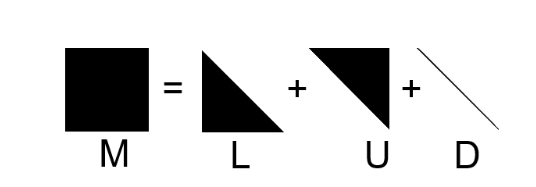
\includegraphics[]{LUD}
        \centering
        \caption{Podział macierzy systemowej w metodach iteracyjnych.(źródło: instrukcja do laboratorium nr 3)}

    \end{figure}

    \noindent Rozpatrzamy układ równań postaci: \\

    $\bm{M}\bm{x} = \bm{b}$ \\

    \noindent Gdzie \textbf{M} jest macierzą systemową, \textbf{x} wektorem rozwiązań i \textbf{b} jest wetkorem współczynników.

    \subsection{Wektor residuum}
    Wektor residuum jest bardzo istotnym elementem metod iteracyjnych.
    Badając jego normę euklidesową możemy okreslić moment, w którym przybliżenie wyniku jest
    zadowalające i algorytm może zakończyć działanie. Zakończenie algorytmy następuje w momencie,
    gdy norma ta jest mniejsza niż podany parametr epsilon.\\

    \noindent Norma euklidesowa wektora x ma postać:

        \[ 
            || x ||_2 = \sqrt{ \sum_{i = 1}^{n} x_i^2} 
       \]


    \subsection{Metoda Jacobiego}

    Podstawiając do powyższego równania \textbf{M} = \textbf{L} + \textbf{D} + \textbf{U}, 
    po przekształceniach otrzymujemy następujący schemat iteracyjny: \\
    
    $\bm{x}^{k+1} = -\bm{D}^{-1}(\bm{L} + \bm{U})\bm{x}^k + \bm{D}^{-1}\bm{b}$ \\

    \noindent k - przybliżenie wyniku po k-tej iteracji

    \newpage

    \noindent Możemy zauważyć, że czynniki $-\bm{D}^{-1}(\bm{L} + \bm{U})$ oraz $\bm{D}^{-1}\bm{b}$
    możemy obliczyć jeden raz, zamiast w każdej iteracji osobno. Obliczenie pierwszego z tych czynników może być
    kosztowne, ponieważ dokonujemy mnożenia dwóch macierzy (złożoność - $O(n^3)$), 
    a nie mnożenia $macierz \times wektor$ (złożoność - $O(n^3)$). W przypadku naszego zadania warto zauważyć,
    że wszystkie elementy na głównej przekątnej macierzy D są takie same.
    Możemy zatem przedstawić macierz D w postaci: $\bm{D} \; = \; d_{00}\bm{I}$, a następnie korzystając z własności 
    macierzy jednostkowej obliczyć nasz czynnik jako: $-\bm{D}^{-1}(\bm{L} + \bm{U}) = -d^{-1}_{00} \cdot (\bm{L} + \bm{U})$.
    Wykorzystamu zatem mnożenie skalarane macierzy zamiast zwykłego, co pozwala
    zoptymalizować działanie algorytmu. \\ 
    
    \noindent Jako, że macierz $\bm{D}$ jest macierzą diagonolną, 
    możemy dokonać jej jawnego odwrócenia bez dużych kosztów pamięciowych: wystarczy elementy na przekątnej zamienić na ich 
    odwrotności. \\
    
    \noindent Po powyższych obliczeniach, działania, które należy wykonać podaczas każdej iteracji to:
    \begin{itemize}
        \item sprawdzenie czy norma wektora residuum jest odpowienio niska, jeżeli nie to:
        \item $ -\bm{D}^{-1}(\bm{L} + \bm{U}) \cdot \bm{x}_{k-1}$ 
        \item $ \bm{x}_k = <wynik \; poprzedniego \; punktu> \; + \; \bm{D}^{-1}\bm{b}$
    \end{itemize}

    \noindent Działania te powtarzamy, aż do uzyskania przybliżenia wyniku, które spełnia nasze oczekiwania co do dokładności.


    \subsection{Metoda Gaussa-Seidla}
    Analogicznie do metody Jacobiego uzyskujemy schemat iteracyjny: \\ 

    $\bm{x}^{k+1} = -(\bm{D} + \bm{L})^{-1}(\bm{U}\bm{x}^k) + (\bm{D} + \bm{L})^{-1}\bm{b}$ \\

    \noindent W metodzie Gaussa-Seidla każda pętla algorytmu jest bardziej kosztowna obliczeniowo niż w przypadku metody Jacobiego.
    Jest to spowodowane faktem, że w metodzie Gaussa-Seidla raz możemy obliczyć tylko jeden wyraz: $(\bm{D} + \bm{L})^{-1}\bm{b}$.
    Jako, że macierz $(\bm{D} + \bm{L})$ jest macierzą dolną trójkątną, możemy w tym celu wykorzystać metodę podstawiania w przód.

    \noindent Pierwszy wyraz, $ -(\bm{D} + \bm{L})^{-1}(\bm{U}\bm{x}^k)$, trzeba obliczać podaczas każdej iteracji.
    W tym przypadku nie mozemy jawnie odwrócić macierzy $(D+L)^{-1}$, ponieważ wiązałoby się to z dużymi kosztami pamięciowymi.
    Musimy więc rozwiązać układ równań liniowych postaci: $ -(\bm{D} + \bm{L})^{-1}(\bm{U}\bm{x}^k)$,
    a następnie do otrzymanego wyniku dodać obliczony na początku algorytmu wyraz. Można zauważyć, że macierz $(\bm{D} + \bm{L})$
    jest macierzą dolną trójkątną oraz wyraz $(\bm{U}\bm{x}^k)$ jest wekotrem. Możemy zatem wykorzystać metodę podstawiania w przód do rozwiązania tego układu.
    


    \subsection{Wyniki obliczeń}
    Rozwiązując układ rówań z zadania A, uzyskane wyniki są następujące:

    \begin{figure}[h]

        \centering
        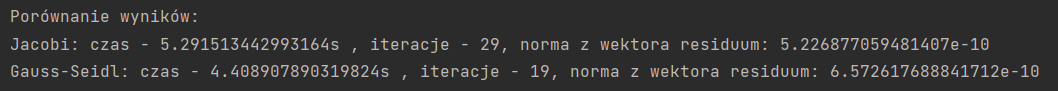
\includegraphics[width=\textwidth]{porownaniGSJac.png}
        \centering
        \caption{Porównanie działania metod iteracyjnych}

    \end{figure}

    Jak widać na powyższym zrzucie ekranu, metoda Jacobiego porzebuje większej liczby iteracji niż metoda Gaussa-Seidla.
    Jednak to metoda Gaussa-Seidla szybciej zakończyła obliczenia. Metoda Gaussa-Seidla jest szybsza i potrzebuje mniej iteracji 
    do uzyskania zadowalającego przybliżenia wyniku. Obie metody działają poprawnie.
    \section{Zadanie C}
    Dane dla zadania C (nr indeksu: 184531):
    \begin{itemize}
        \item $a_1 = 3$ 
        \item $a_2 = a_3 = -1$
        \item $N = 931$
    \end{itemize}

    \noindent Wygenerowana macierz systemowa C (o rozmiarze $931 \times 931$): \\

    %tutaj macierz z zadania A
    $\begin{bmatrix}
    3 & -1 & -1 & 0 & 0 & 0 & 0 & \ldots & 0 \\
    -1 & 3 & -1 & -1 & 0 & 0 & 0 & \ldots & 0 \\
    -1 & -1 & 3 & -1 & -1 & 0 & 0 & \ldots & 0 \\
    0 & -1 & -1 & 3 & -1 & -1 & 0 & \ldots & 0 \\
    0 & 0 & -1 & -1 & 3 & -1 & -1 & \ldots & 0 \\
    0 & 0 & 0 & -1 & -1 & 3 & -1 & \ldots & 0 \\
    0 & 0 & 0 & 0 & -1 & -1 & 3 & \ldots & 0 \\
    \vdots & \vdots & \vdots & \vdots & \vdots & \vdots & \vdots & \ddots & \vdots \\
    0 & 0 & \ldots & 0 & 0 & 0 & -1 & -1 & 3
    \end{bmatrix}$
    \\ 

    \noindent Za generowanie macierzy oraz wektora współczynników B odpowiadają
    odpowiednie funckje w module Functions.py

    \noindent Metody iteracyjne dla tej macierzy nie zbiegają się. W przypadku metody Gaussa-Seidla wynika
    to prawdopodobnie z faktu, że macierz \textbf{C} nie jest dodatnio określona, a w przypadku metody
    Jacobiego z faktu, że promień spektralny macierzy $\bm{D}^{-1}(\bm{L} + \bm{U})$ jest większy niż 1.

    \newpage
    \section{Zadanie D}
    W faktoryzacji LU przedstawiamy macierz systemową w postaci iloczynu dwóch macierzy trójkątnych. \\

    $\bm{A} = \bm{L}\bm{U}$ \\

    \noindent Gdzie \textbf{L} to macierz trójkątna dolna, zawierającą na przekątnej 1 i \textbf{U} to macierz trójkątna dolna.
    Najbardziej kosztowną operacją w metodzie LU jest uzyskanie macierzy \textbf{L} i \textbf{U}.

    \noindent Gdy dokonamy już faktoryzacji macierzy \textbf{A}, wykonujemy następujące działania:
    \begin{itemize}
        \item $\bm{L}\bm{U}\bm{x} = \bm{b}$
        \item tworzymy wektor pomocniczy: $\bm{y} = \bm{U}\bm{x}$
        \item rozwiązujemy układ równań: $\bm{L}^{-1}\bm{b} = \bm{y}$ metodą podstawiania w przód
        \item rozwiązujemy układ równań: $\bm{U}^{-1}\bm{y} = \bm{x}$ metodą podstawiania w tył
    \end{itemize}

    \noindent Metoda ta ma złożoność obliczeniową $O(n^3)$. Zaletą faktoryzacji LU jest fakt, 
    że w przypadku gdy chcemy rozwiązać układ równań dla wielu prawych stron i tej samej macierzy 
    systemowej, ponieważ najbardziej kosztowną część algorytmu - dekompozycje macierzy - wystarczy 
    wykonać jeden raz.

    \begin{figure}[h]

        \centering
        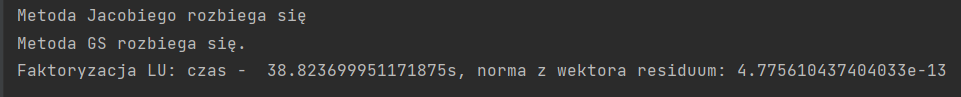
\includegraphics[width=\textwidth]{LU.png}
        \centering
        \caption{Zadanie C - jak widać metody iteracyjne rozbiegają się}

    \end{figure}

    \noindent Norma z wektora residuum wynosi ok. $4.8 \cdot 10^{-14} $, 
    a więc jest ok. $10^5 $ razy niższa niż w przypadku metod iteracyjnych, jednak zwróćmy uwagę,
    że w ich przypadku moglibyśmy podać jako epsilon np. $10^{-16}$ i wtedy rozwiązanie byłoby dokładniejsze.
    
    \noindent Jednak metody bezpośrenie charakteryzują się tym, że dadzą nam wynik po określonej liczbie operacji,
    podczas gdy metody iteracyjne mogą się rozbiegać.
    \newpage
    \section{Zadanie E}
    Utworzyłem wykres dla liczby zmiennych N = {100, 500, 1000, 2000, 3000}.
    W celu lepszego ukazania różnić między metodami na osi y użyłem skali logarytmicznej.


    \begin{figure}[h]

        \centering
        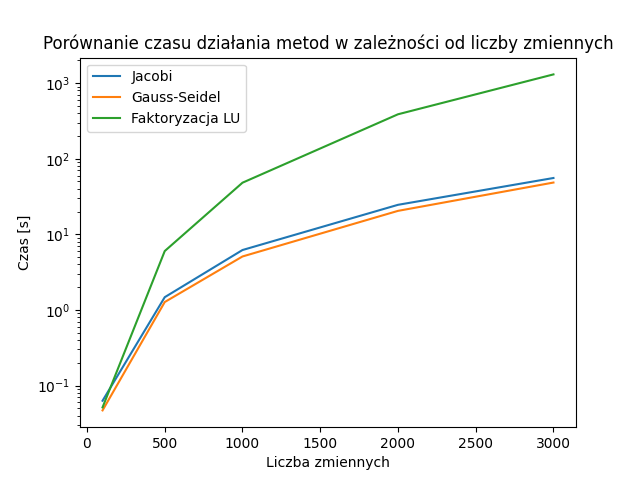
\includegraphics[width=\textwidth]{test.png}
        \centering
        \caption{Zadanie E - wykres czasu działania różnych metod}

    \end{figure}
    \newpage
    \section{Zadanie F}
    Analizując powyższy wykres możemy zauważyć, że metoda faktoryzacji LU jest znacząco wolniejsza
    niż obie metody iteracyjne.
    \begin{figure}[h]

        \centering
        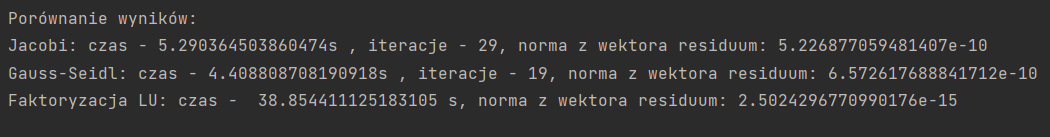
\includegraphics[width=\textwidth]{LUJacGS.png}
        \centering
        \caption{Porównanie czasów działania dla układu z zadania A}

    \end{figure}

    \noindent Gdy uruchomimy wszystkie 3 metody na układzie z zadania A, 
    wyniki odzwierciedlają to co widzimy na wykresie - dla 931 zmiennych najszybsza jest metoda 
    Gaussa-Seidla, niewiele wolniejsza jest metoda Jacobiego, a metoda faktoryzacji LU potrzebuje 
    znacznie więcej czasu do uzyskania wyniku. Metoda Jacobiego potrzebuje więcej iteracji niż metoda
    Gaussa-Seidla, ale działa podobnie szybko. Iteracje metody Gaussa-Seidla są bardziej kosztowne,
    ponieważ w każdej iteracji musimy dokonać mnożenia macierzy przez wektor.

    \noindent Warto jednak zauważyć, że faktoryzacja LU uzyskuje znacznie dokładniejszy wynik.
    Tak dokładny wynik rzadko jest nam potrzebny, a w metodach iteracyjnych możemy 
    sterować dokładnością przez parametr epsilon.

    \noindent Przeprowadziłem eksperyment i ustawiłem jako epsilon dla metod iteracyjnych wartośc $10^{-14}$,
    czyli taką samą jak daje faktoryzacja LU.

    \begin{figure}[h]

        \centering
        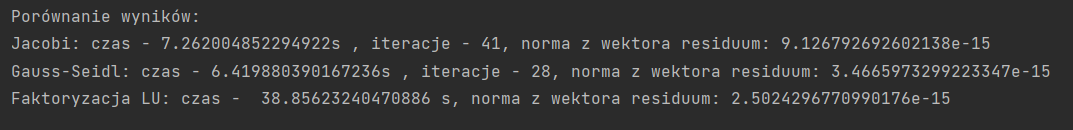
\includegraphics[width=\textwidth]{tasamadok.png}
        \centering
        \caption{Czasy działania przy takiej samej dokładności wyniku}

    \end{figure}

    \noindent Jak widać po wynikach, metody iteracyjne są znacznie szybsze,
    nawet przy takiej samej dokładności. Jest to maksymalna dokładność z jaką możemy uzyskać
    wynik dla metod iteracyjnych. Przy wartościach niższych metody rozbiegają się.
    
    \section{Porównanie z biblioteką Numpy}
\end{document}_